\documentclass[conference]{IEEEtran}

\usepackage{graphicx}
\usepackage{url}
\usepackage{cite}

\hyphenation{op-tical net-works semi-conduc-tor net-works MA-NET through meth-odologies}


\begin{document}

\title{AD-ZRP: Ant-based Routing Algorithm for Dynamic Wireless Sensor Networks}

\author{
    \IEEEauthorblockN{Alexandre Massayuki Okazaki and Ant\^onio Augusto Fr\"ohlich}
    \IEEEauthorblockA{
        Laboratory for Software and Hardware Integration (LISHA)\\
            Federal University of Santa Catarina (UFSC)\\
            P.O.Box 476, 88040900 -- Florian\'opolis -- Brazil\\
            \{alexandre,guto\}@lisha.ufsc.br
    }
}

\maketitle

\begin{abstract}
In this paper, we introduce Ant-based Dynamic Zone Routing Protocol (AD-ZRP), a self-configuring reactive routing protocol for Wireless Sensor Networks (WSNs).
Our approach is based on HOPNET, a multi-hop and self-configuring hybrid routing protocol based on Ant Colony Optimization (ACO) and Zone Routing Protocol (ZRP) for Mobile Ad Hoc Networks (MANETs).
There are many challenges in designing routing protocols for WSNs, and topology change is a factor that affects the network lifetime of WSNs.
And with the robustness of routing protocols for MANETs, dealing with dynamic topologies becomes a less arduous task.
However, WSNs tend to be more stringent than MANETs in respect to resource availability, then the AD-ZRP design must consider several restrictions including energy consumption, processing power, memory, and bandwidth.
AD-ZRP also consists of ZRP, but it is based on dynamic zones which, acting together with ACO, allows us to deal with the restrictions of WSNs and yet improve the route discovery and the route maintenance through pheromone.
We have evaluated and compared our algorithm to the original HOPNET and obtained better results in terms of data delivery ratio, routing overhead, and congestion avoidance for environments of dynamic topology.
\end{abstract}

\IEEEoverridecommandlockouts
\IEEEpubid{978-1-4577-0024-8/11/\$26.00~\copyright2011 IEEE}
\IEEEpubidadjcol
%\IEEEpeerreviewmaketitle

\section{Introduction}
\label{introduction}

WSN is a class of wireless ad hoc network which consists of a set of sensor nodes.
It aims at several applications such as home automation, industrial sensing and control, and environment monitoring \cite{Shuang:2009}.
Sensor nodes are characterized by their constraints in processing power, memory, bandwidth, and energy consumption \cite{Matrouk:2009}.
They are often deployed in harsh environments.
As a result, node damage and failure become common events.
Therefore, associated routing protocols must handle network topology changes dynamically.
This adds to the typical topology change of MANETs due to node mobility \cite{Garcia:2007}.
Moreover, by introducing mobility to WSNs, the network capability can be improved in many aspects, such as automatic node deployment, flexible topology adjustment, and rapid event reaction \cite{Wang:2010}.
This way, routing algorithms for WSNs which handle the overhead of topology changes and mobility have attracted a significant interest \cite{Akkaya:2005}.

WSNs are noisy and error-prone, as a result, many routing techniques attempt to obtain reliable routes.
Therefore, several solutions monitor the quality of links using metrics such as signal strength, data reception ratio, location, and heuristics in order to maintain reliable links between nodes \cite{Stankovic:2008}.
Moreover, routing algorithms inspired by ant collective intelligence can be an effective way to deal with dynamic topologies due to the ability of ants to perceive changes in networks through pheromone.

In this paper, we introduce a new routing method based on \emph{dynamic zones}.
It is inspired by ZRP and allows us to deal with the overhead of dynamic topologies taking into account congestion and unreliable links between nodes.
We also designed AD-ZRP, a self-configuring reactive routing protocol.
It is based on the HOPNET algorithm, a multi-hop hybrid routing protocol inspired by ACO and ZRP for MANETs \cite{Wang:2009}.
ACO-based routing protocols usually provide the ability to learn the shortest routes \cite{Lu:2004} and yet automatically adapt to network topology changes \cite{Iyengar:2007}.
Routing algorithms with such characteristics have been considered as an alternative for many scalable multi-hop networks, including WSNs \cite{Okdem:2009, Dhurandher:2009}.
With the robustness of HOPNET and the \emph{dynamic zones} method, AD-ZRP allows us to improve the route discovery and maintenance through pheromone.
It helps us to handle important routing problems in ad hoc networks such as route discovery and broken routes.
These contributions allow us to achieve a routing algorithm powerful enough to ensure reliable routes among nodes to handle congestion in dynamic topology environments like MANETs.
However, several routing schemes of MANETs are inadequate for WSNs due to typical limitations of sensor network nodes \cite{Okdem:2009}.
Hence, these constraints were taken in consideration in the design of our routing algorithm in order to achieve a suitable protocol for WSNs.

The remainder of this paper is organized as follows: section \ref{related} presents related work.
In section \ref{proposed_scheme}, we explain and describe AD-ZRP.
In section \ref{evaluation}, we evaluate our implementation.
Finally, we present our conclusion of the study in the last section.

\section{Related Work}
\label{related}
\IEEEpubidadjcol

HOPNET is a self-configuring routing technique based on zones and inspired by ant collective intelligence in order to obtain reliable routes between nodes in ad hoc networks \cite{Wang:2009}.
ZRP is a hybrid routing protocol which aims to reduce the control overhead of proactive protocols and the latency of reactive protocols \cite{Haas:1997}.
In ZRP, each node maintains a zone in order to obtain reliable link information among its neighbors through proactive routing.
Moreover, the data to nodes beyond the zone are routed through reactive routing.
Different from ZRP, HOPNET involves ant collective intelligence in the proactive routing to maintain and improve the existing routes or explore better options.

Nevertheless, HOPNET is not a suitable routing protocol for WSNs.
The main challenges of routing in WSNs are to support data communication while trying to prolong the lifetime of nodes' batteries, prevent connectivity degradation, decrease congestion, and improve energy efficiency.
In many address-based routing protocols, such as most of the routing protocols for MANETs, there is a lack of global identification along with random deployment of sensor nodes which makes it hard to select a specific set of nodes to be queried \cite{Akkaya:2005}.
Therefore, routing protocols for WSNs that are able to select a set of sensor nodes and perform aggregation during the relaying of data have also been considered to reduce the transmitted redundant data.
However, differently from our proposal, most of these protocols do not consider dynamic network topologies.

\emph{Adaptive Ant Colony System} (AACS) is a data-centric routing protocol which uses \emph{Direct Diffusion} to distribute interest messages and applies the AACS algorithm to construct the \emph{Minimum Steiner Tree} (MST) \cite{Li:2008}.
Data-aggregation based on AACS, along with the MST, helps to reduce the amount of transmitted data in the network aiming at saving energy and prolonging network lifetime.
Nonetheless, in dynamic network topologies, the algorithm needs to reconstruct the MST periodically causing additional overhead and thus compromising both targeted metrics.

\emph{Ant-Based On-Demand Energy Route} (AOER) is  a routing algorithm for IEEE 802.15.4 mesh networks \cite{Shuang:2009}.
Different from other protocols based on ACO, AOER requires less memory storage, less processing power, and uses simpler data structures for ants and routing table.
The algorithm maintains the routes by inserting pheromone according to the residual energy in the nodes in order to equally distribute the traffic in the network.
AOER has shown good results in prolonging the network lifetime and balancing energy consumption among nodes.
The authors present a solution similar to our approach taking into account the reduction of memory and processing.
However, AOER uses a mechanism to proactively maintain routes which tends to increase the overhead considerably in networks with high scalability.
Different from our proposal, which belongs to the class of reactive protocols and uses \emph{dynamic zones} to deal with the overhead and latency.

Vlajic and Stevanovic \cite{Vlajic:2009} analyzed the pros and cons of deploying path-constrained mobile sinks in real IEEE 802.15.4 networks.
They introduced two simple mechanisms for the reduction of mobility-related overhead in WSNs.
They also demonstrated analytically and through simulation that in idealist networks, mobile sinks can result in a better distribution of routing load and longer network lifetime.
Unfortunately, in real world networks, including IEEE 802.15.4, the overhead is not zero.
These networks use mechanisms that generate additional overhead to manage congestion, lessen mobility, and consequently bring down the amount of changes in network topology.
Hence, for contemplating the use of real WSNs with continuous changes in network topology, the minimization of protocol overhead may have to be the first course of action.

\section{AD-ZRP: The Proposed Routing Scheme}
\label{proposed_scheme}

Our proposal, AD-ZRP, is a self-configuring and multi-hop reactive routing protocol based on the HOPNET algorithm.
With the robustness of HOPNET, our approach handles important problems in ad hoc networks to improve the discovery and maintenance of routes through ACO and ZRP features.

In the real world, ants communicate with each other using pheromone.
Each one takes a random walk from its anthill to search for some kind of food.
Ants indiscriminately follow many different ways in accordance with their level of pheromone.
On the way back to the anthill, they deposit pheromone on the track to allow other ants to find the leftover food thus reinforcing the pheromone on the trail.
Hence, the reinforcement in shorter tracks tends to be more attractive.
However, over the course of time, the pheromone on the trail will gradually evaporate.
As a result, when the food runs out, new trails are not marked by returning ants, and the pheromone slowly dissipates.
This behaviour helps ants to deal with changes in their environment.

\begin{figure*}[htb]
\centering
\begin{tabular}{c c c}
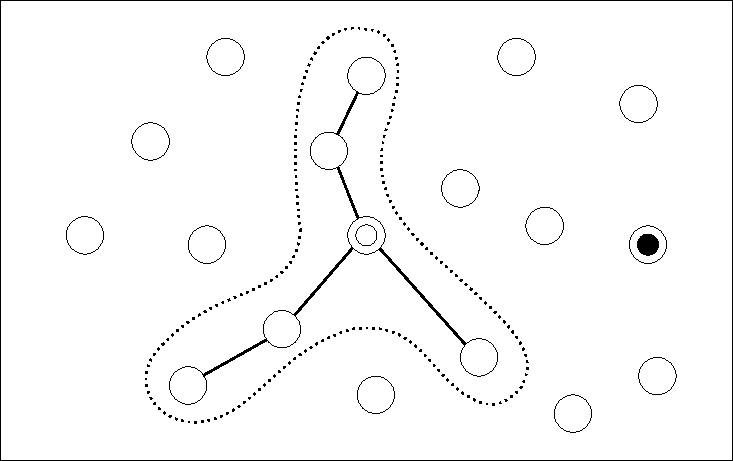
\includegraphics[width=140pt]{fig/dynamic_zone_part_1.pdf} &
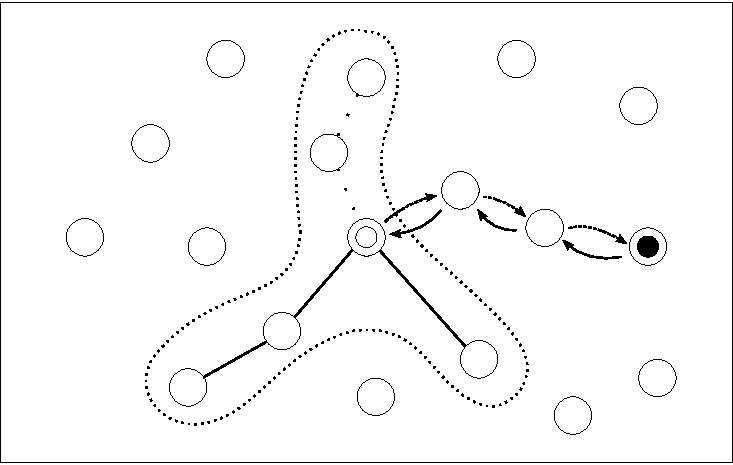
\includegraphics[width=140pt]{fig/dynamic_zone_part_2.pdf} &
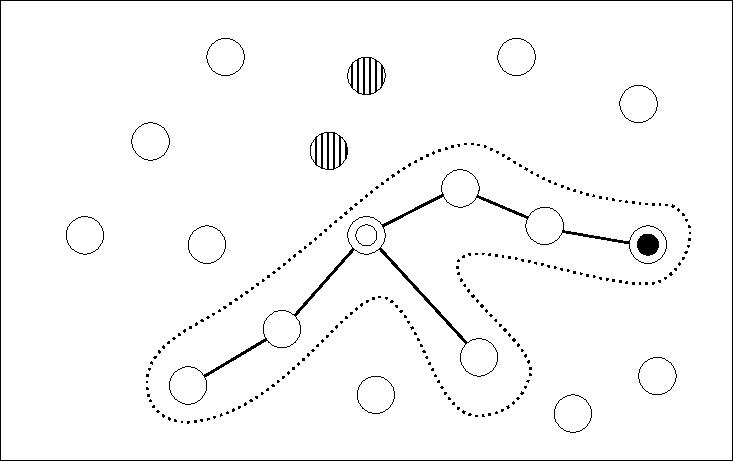
\includegraphics[width=140pt]{fig/dynamic_zone_part_3.pdf} \\
\multicolumn{3}{c}{ 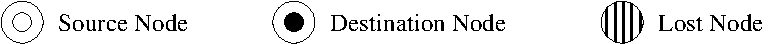
\includegraphics[width=200pt]{fig/dynamic_zone_subtitle.pdf} } \\
(a) & (b) & (c) \\
\end{tabular}
\caption{Dynamic Zone - Interzone Routing Discovery}
\label{dynamic}
\end{figure*}

ACO is a technique based upon using ant collective behavior to solve computational problems \cite{Dorigo:2005, Dorigo:2006}.
The idea behind routing protocols based on ACO is to apply it to discover and maintain the best routes among the nodes.
These protocols can thereby maintain the routing table efficiently updated due to the proportionate dynamism of ants to adapt, by pheromone, to topology changes.

In HOPNET, if most of the transmissions are performed between nodes that share the same zone, then each source node can quickly obtain routes to any destination by \emph{Intrazone Routing Tables} (IntraRT).
It is a table whose rows represent its neighbors and the columns represent all identified nodes within its zone, similarly to the inverted pheromone table of AOER \cite{Shuang:2009}.
All ants have the responsibility to maintain the IntraRTs proactively within their zones by mapping and reinforcing the best routes through pheromone.
Nonetheless, if most of the transmissions are to nodes outside the zone, then the routing becomes expensive.
In order to transmit or relay the data packets, each source node must first check the \emph{Interzone Routing Table} (InterRT) to use a route already discovered.
It is a routing table responsible for storing the path travelled by ants, from the source to the destination, when the destination is an unknown node or a node out of zone.
If the external node is not in InterRT, then the source node need start a search process to discover a new route to the external node.
However, if the external node is not in InterRT as a destination, but it is part of any route, then each route in InterRT has to be minutely verified in order to find the route to this node.
In both cases, there is waste of memory and processing.
In order to reduce the on-demand data transmissions, HOPNET allows us to increase the zone radius to enlarge the zone and thus increasing the amount of nodes within the zone \cite{Wang:2009}.
Nonetheless, defining an optimal zone radius for each network is a challenge.
If the zone is too large and dense, the overhead increases in the network, such as in proactive routing protocols.
On the other hand, if the zone is too small and sparse, the latency increases, such as in reactive routing protocols.

Nevertheless, AD-ZRP is proposed as a reactive routing protocol to avoid sending ants periodically into their zones and thus bringing additional overhead to the sensor network.
Different from HOPNET, which uses fixed-sized zones defined by the zone radius, our approach uses \emph{dynamic zones} to minimize the latency while reducing the network overhead.
\emph{Dynamic zones} change their shape and size almost constantly since the zones vary according to on-demand transmissions.
They are defined by the presence of pheromone on routes between the source nodes and any other node in the network.
Initially, when there is no pheromone distributed over the network, all zones are empty.
After each data packet transmission to an unknown destination, a new route is added to the zone.
Meanwhile, if some routes are no longer used, then they may eventually leave the zone due to evaporation.
Figure \ref{dynamic} shows the behavior of a \emph{dynamic zone} when a new route is discovered and introduced as part of the zone, and when another route leaves it.
In Figure \ref{dynamic} (b), the process basically starts with the transmission of an ant to find a route to the destination.
This way, new routes can be added to the zone while others may leave it due to the links between nodes whose pheromone has been exhausted, as shown in Figure \ref{dynamic} (c).

While HOPNET uses two routing tables to perform intrazone and interzone routing separately, our proposal uses only IntraRT as routing table structure.
Different from InterRT, its operations are simpler and faster, and routes beyond the zones do not need to be stored entirely.
Both intrazone and interzone routing can thereby use the same structure and the same operations to deal with dynamic changes along the routes that must be accomplished only by way of pheromone.
In order to accomplish these routing operations, a new collection of ants is presented: \emph{internal transport ant} (ITA) and \emph{exploratory transport ant} (ETA).
Although each ant category has a different function, they share a common data structure.
Figure \ref{ad-zrp_protocol} shows the ant data structure of AD-ZRP.

\begin{figure}[htb]
\centering
\begin{tabular}{c}
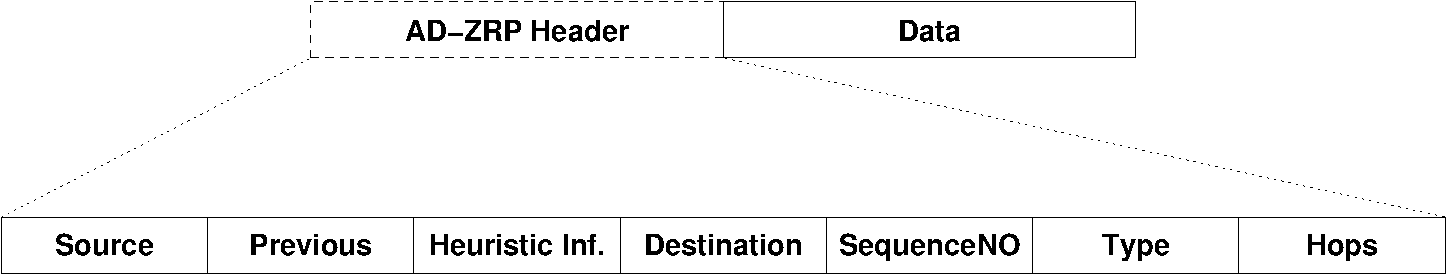
\includegraphics[width=235pt]{fig/ad-zrp_protocol.pdf}
\end{tabular}
\caption{AD-ZRP Ant Structure}
\label{ad-zrp_protocol}
\end{figure}

The ant structure includes address fields as \emph{Source} and \emph{Destination}.
The \emph{Previous} field is responsible for storing the address of the previous node.
The \emph{Heuristic Inf.} field is responsible for storing the necessary heuristic information to calculate the pheromone deposit ratio.
The \emph{SequenceNO} field is used for control.
The \emph{Type} field indicates the ant category, and the \emph{Hops} field indicates the number of hops that the ant has done.

These ants help to reduce the complexity to offer better tactics to diffuse and verify pheromone among the nodes, reinforcing the links between neighbors to maintain the best routes in the zone according to the heuristic information.
In addition, both ITA and ETA perform data delivery while they deposit pheromone on the route which they travel.

In HOPNET, if there is any change in the route during data transmission, \emph{notification ants} and \emph{error ants} are sent to notify the other nodes and get a new route, thus causing additional overhead to the network.
Hence, in AD-ZRP, the data packet is sent along with the ant to ensure that sudden changes in the network do not interfere with the transportation of the data towards the destination.
The data packet may thereby be dynamically redirected to a safer route.
Figure \ref{ad-zrp_data_tx} depicts the activity diagram for data transmission in AD-ZRP.

\begin{figure}[htb]
\centering
\begin{tabular}{c}
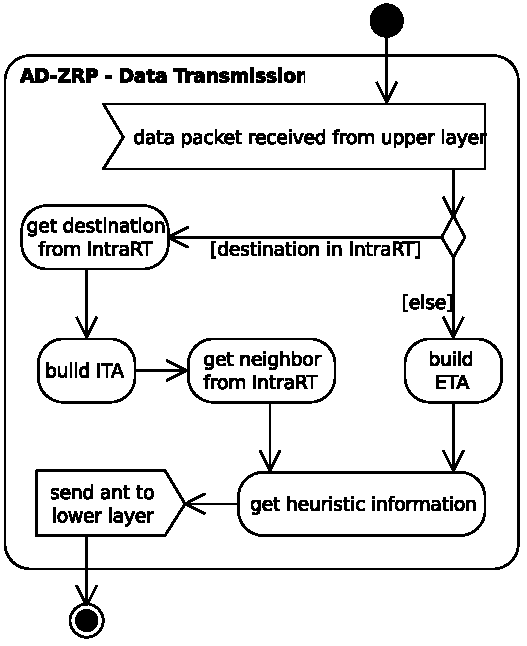
\includegraphics[width=160pt]{fig/ad-zrp_data_tx.pdf}
\end{tabular}
\caption{Data Transmission}
\label{ad-zrp_data_tx}
\end{figure}

ETAs are responsible for discovering routes to unknown nodes.
These ants travel through the network to discover the destination node.
At the destination, the ETA delivers the data packet and returns to the source node.
On the way back, the ant just sets the pheromone trail in order to add it to the zone, as shown in Figure \ref{ad-zrp_rx_eta}.

\begin{figure}[htb]
\centering
\begin{tabular}{c}
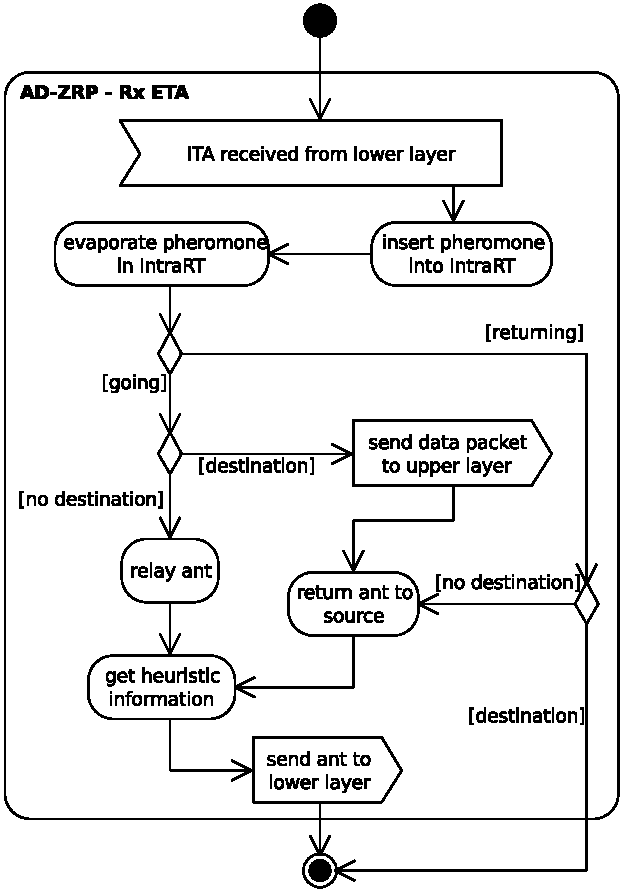
\includegraphics[width=170pt]{fig/ad-zrp_rx_eta.pdf}
\end{tabular}
\caption{Rx ETA}
\label{ad-zrp_rx_eta}
\end{figure}

ITAs are responsible for delivering data packets only within their zone.
When a source node discovers a new route to certain destination by ETA, the following data packet transmissions are performed by ITAs until the pheromone amount on the route evaporates entirely.
Nevertheless, at any time, if any route to any destination breaks, any node on the route can use an ETA to recover it or discover a new path, as the activity diagram shown in Figure \ref{ad-zrp_rx_ita}.

\begin{figure}[htb]
\centering
\begin{tabular}{c}
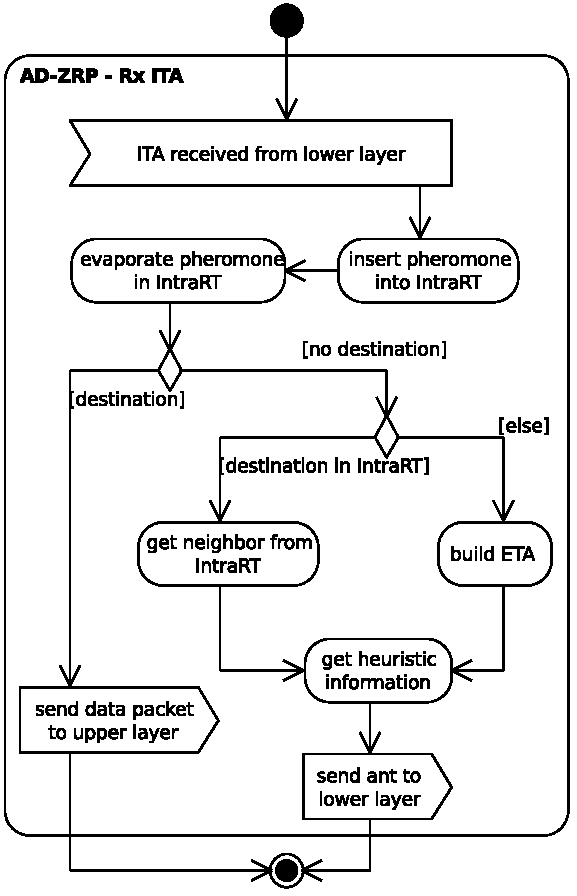
\includegraphics[width=170pt]{fig/ad-zrp_rx_ita.pdf}
\end{tabular}
\caption{Rx ITA}
\label{ad-zrp_rx_ita}
\end{figure}

Different from HOPNET, our approach uses different equations for deposit and evaporation of pheromone.
Each ant selects a node $v_{j}$ as the next hop from the current node $v_{i}$.
At the node $v_{j}$, the ant updates the pheromone $\tau _{i,s}$ on the entry $\left ( v_{i},v_{s} \right )$ in IntraRT, where $v_{s}$ is the source node, as follows \cite{Dorigo:2006}:
\begin{equation} \tau _{i,s} = \left ( 1 - \varphi \right ) \cdot \tau _{i,s} + \varphi \cdot \tau _{0} \label{ad-zrp_pheromone_increasing} \end{equation}
where $\tau _{0}$ is the initial value of pheromone, and $\varphi \in \left ( 0,1  \right ]$ is the pheromone decay coefficient which is calculated from the heuristic information (Figure \ref{ad-zrp_protocol}) of the node $v_{i}$.

The equation (\ref{ad-zrp_pheromone_increasing}) allows us to diversify the search process by increasing or decreasing the pheromone amount in the routes while allowing other ants to achieve different routes.
It also helps to increase the effect of \emph{dynamic zones}, allowing us to deal with dynamic network topologies and avoid as much as possible broken routes.

The evaporation occurs periodically to all nodes in the network, using the following equation:
\begin{equation} \tau _{i,j} = \left ( 1 - \rho \right ) \cdot \tau _{i,j} , \quad \forall i \in N, \quad \forall j \in Z \label{evaporation} \end{equation}
where $\rho \in \left ( 0,1  \right ]$ is the evaporation ratio, $N$ is the set of neighbor nodes, and $Z$ is the set of nodes which, together with neighbor nodes, define entries $\left ( v_{i},v_{j} \right )$ in IntraRT.


\section{Performance Evaluation}
\label{evaluation}

In order to analyze the changes made and compare the performance between AD-ZRP and HOPNET, we evaluated both algorithms in a simulation environment.
The implementations were performed using the \emph{Global Mobile Information System Simulator} (GloMoSim).
It is a protocol simulation software for network systems that supports routing protocols for purely ad hoc wireless networks.
The evaluation took place by way of a number of simulation scenarios.

Each simulation scenario was run for a total of 900 seconds in an environment that is conducive to high data loss.
The nodes were placed randomly in a rectangular area of 700 meters x 400 meters, and each one moved at a maximum speed of 10 meters per second, according to the \emph{Random Way Mobility Model} (RWP).
The data traffic was generated by 20 \emph{Constant Bit Rate} (CBR) sources.
\emph{User Datagram Protocol} (UDP) supported the network at the \emph{Transport} layer.
\emph{Internet Protocol} (IP) protocol operated at the \emph{Network} layer.
The protocol used for \emph{Data Link} layer and MAC sublayer was the standard IEEE 802.11.
The radio transmission power was set to 15 dBm and the bit rate was 2 megabits per second.
This base scenario was used for the experiments on GloMoSim by varying specific parameters, such as number of nodes and zone radius.
The number of nodes ranged from 20 to 200, and the zone radius ranged from 2 to 5.

Figure \ref{data_delivery_ratio} shows the data packet delivery ratio in this simulation environment.
As the number of node increases, the delivery ratio also increases due to the ants which are able to take the best routes to certain destinations.
If the network is too large and dense, then the delivery ratio is higher due to the large number of routes choices.
On the other hand, if the network is small and sparse, then the delivery ratio decreases due to lack of connectivity among the nodes.
Our approach shows better results of data delivery ratio for networks with high scalability and high mobility.
However, we notice from the figure that both protocols give a low delivery ratio in the simulations of 100 nodes.
We ascribe it to the congestion, as a result of the mobility and placement of nodes at some point in the simulation.

\begin{figure}[htb]
\begin{tabular}{c}
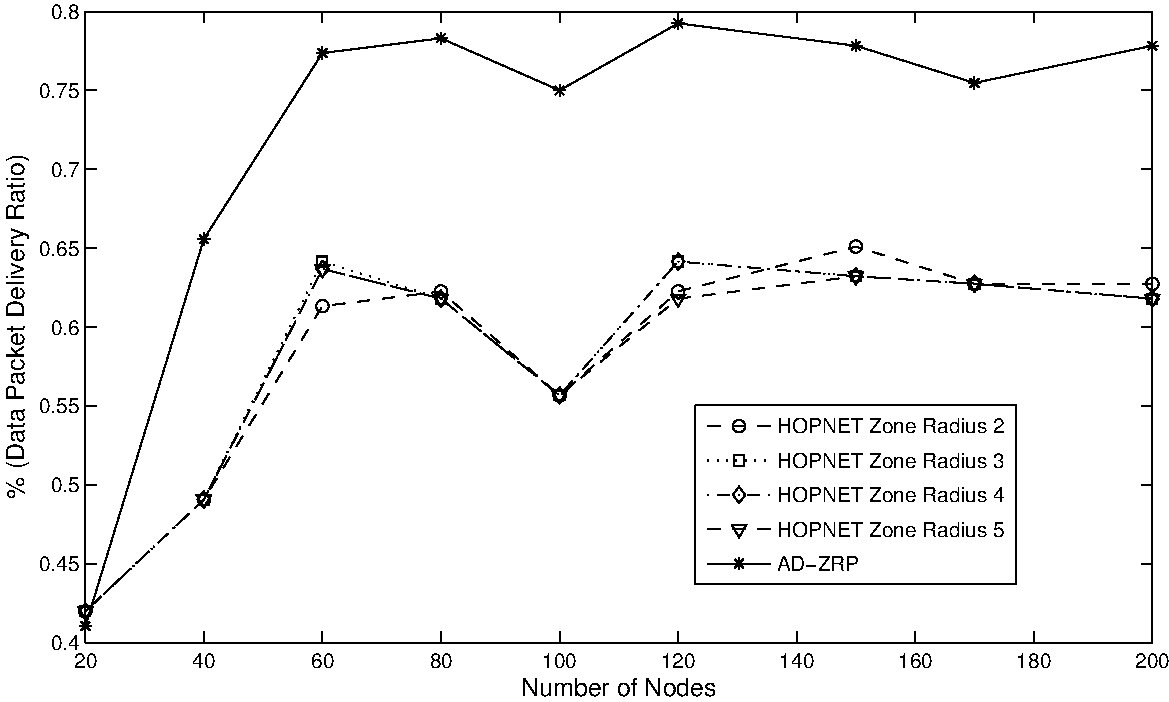
\includegraphics[width=245pt]{fig/data_delivery_ratio.pdf}
\end{tabular}
\caption{Data Packet Delivery Ratio}
\label{data_delivery_ratio}
\end{figure}

HOPNET and AD-ZRP lose data packets in two ways:
\begin{itemize}
\item
through broken routes, due to problems of relaying the received packets along routes that no longer exist;
\item
through link failures, due to problems of connectivity among the nodes.
\end{itemize}

The difference is that in the first case, both HOPNET and AD-ZRP identify and handle the routing errors.
In the second case, the errors are identified by the MAC layer, and through link failure messages, the routing protocol handles them.

Figure \ref{broken_routes} shows the dropped packet ratio due to broken routes.
Because of the low connectivity of small and sparse networks, the data packets cannot be transmitted and the packet loss tends to be low.
Nevertheless, as the number of nodes in the network increases, the amount of broken routes tends to decrease slightly.
Because of the ability of ants to determine the best route between several options to obtain reliable links between nodes along the routes.
Since the routing in AD-ZRP is solely performed by pheromone, the nodes become more attentive as the topology changes.
It also allows us to use more efficient ways to retrieve a route or discover another (Figure \ref{ad-zrp_rx_ita}).
This way, we can notice that our proposal produces better results of broken routes than HOPNET.

\begin{figure}[htb]
\begin{tabular}{c}
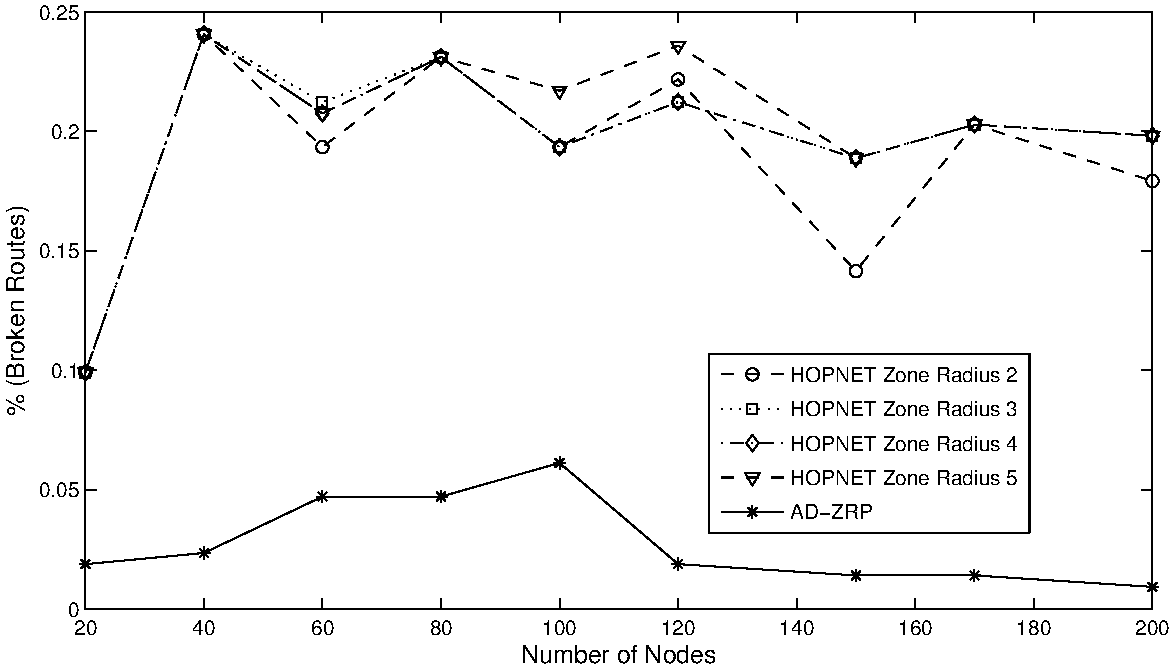
\includegraphics[width=245pt]{fig/broken_routes.pdf}
\end{tabular}
\caption{Broken Routes}
\label{broken_routes}
\end{figure}

If we consider congestion in the simulations of 100 nodes due to mobility and placement of the nodes, then the packet loss due to broken routes tends to be slightly lower in low mobility scenarios.
Figure \ref{broken_routes-speed} shows the results of broken routes by varying the maximum speed of nodes from 1 to 15 meters per second.
We notice from the figure that HOPNET tends to produce significantly better results in networks of low mobility; however, AD-ZRP shows better results than HOPNET, even in scenarios of high congestion where speed is 10 meters per second.

\begin{figure}[htb]
\begin{tabular}{c}
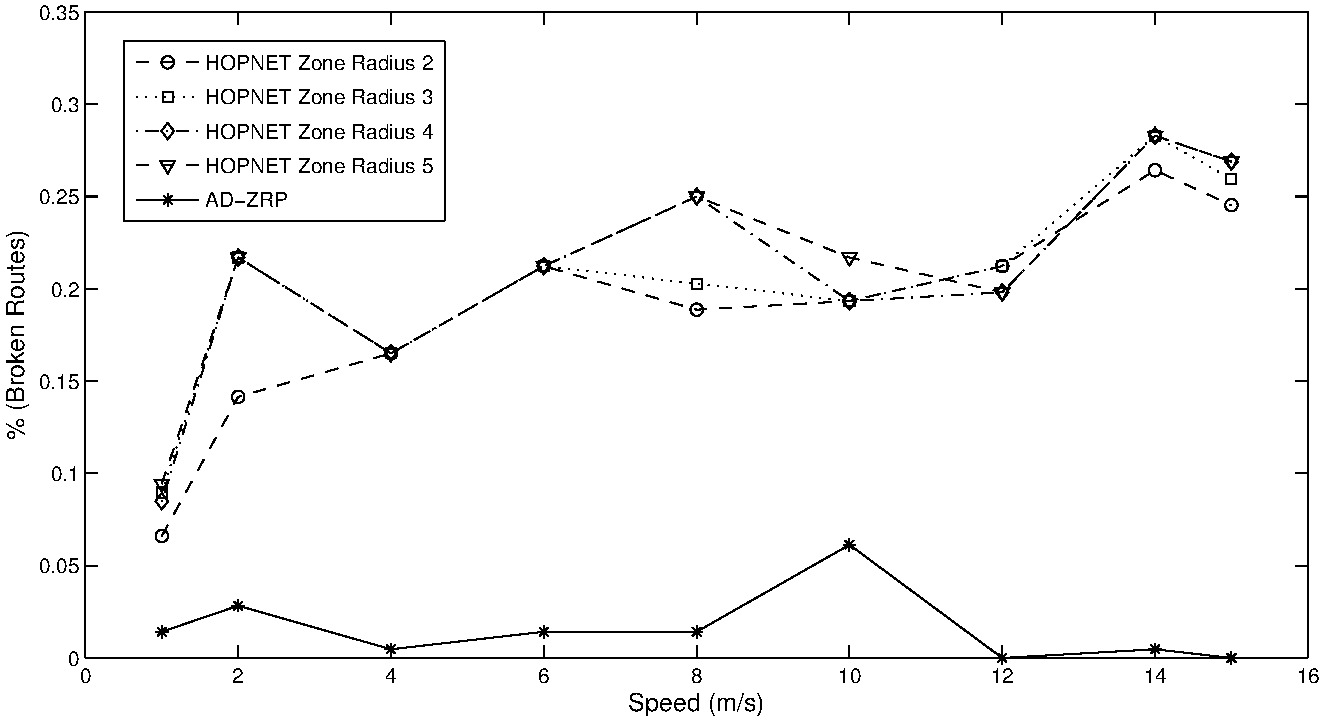
\includegraphics[width=245pt]{fig/broken_routes-speed.pdf}
\end{tabular}
\caption{Broken Routes (100 nodes)}
\label{broken_routes-speed}
\end{figure}

Figure \ref{link_failures} shows the results of dropped packets ratio due to link failures.
Different from broken routes, link failures refers to the error messages that originate from MAC sublayer.
In MAC, if a node does not receive \emph{Clear to Send} (CTS) or \emph{Acknowledgment} (ACK) after several attempts, a link failure message is sent to the routing protocol in order to conduct a repair procedure.
We see from the figure that the amount of link failures is superior in small and sparse networks due to low connectivity between nodes.
We also notice that HOPNET produces better results of link failures than AD-ZRP.
Since our approach is a reactive routing protocol, the links between neighbor nodes tend to be more susceptible to failure.
Because HOPNET has more reliable pheromone information in the zones than AD-ZRP due to proactive routing.
However, our proposal provides better results in situations of congestion and high mobility due to \emph{dynamic zones} which provide better adaptability to dynamic topologies than fixed-sized zones.
Accordingly, the routes reactively discovered are no longer stored as sequences of nodes, and the nodes moving to beyond the zone will not lose the communication due to the zone radius.

\begin{figure}[htb]
\begin{tabular}{c}
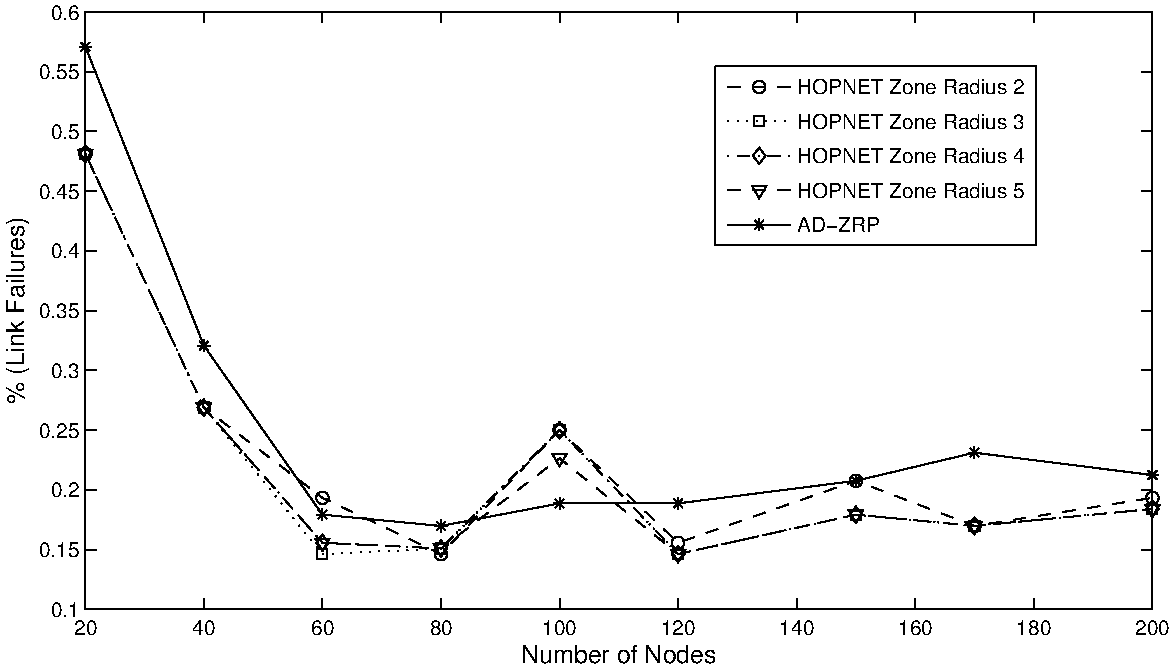
\includegraphics[width=245pt]{fig/link_failures.pdf}
\end{tabular}
\caption{Link Failures}
\label{link_failures}
\end{figure}

Figure \ref{routing_overhead} shows the comparison between HOPNET and AD-ZRP for routing overhead.
In HOPNET, the control packets (ants) are periodically sent out within a zone to maintain the routes in the zone, others are sent out to perform interzone route discovery and repair procedures.
In AD-ZRP, the data is sent along with the ants thereby decreasing the amount of control packets in the network.
We notice from the figure that AD-ZRP gives lower routing overhead than HOPNET due to a reduction of ants in the network.
Accordingly, our approach tends to produce low routing overhead for sparse networks due to low connectivity.
However, it also produces high link failures, as explained in the previous figure.
Differently, HOPNET produces high routing overhead for sparse networks.
On this account, it tends to send many more control packets to obtain reliable routes.
And as the number of nodes increases, the routing overhead also tends to increase.
In another way, since the data is sent along with the ants and the routing is reactive, the routing overhead of our proposal tends to stay almost constant for large and dense networks.

\begin{figure}[htb]
\begin{tabular}{c}
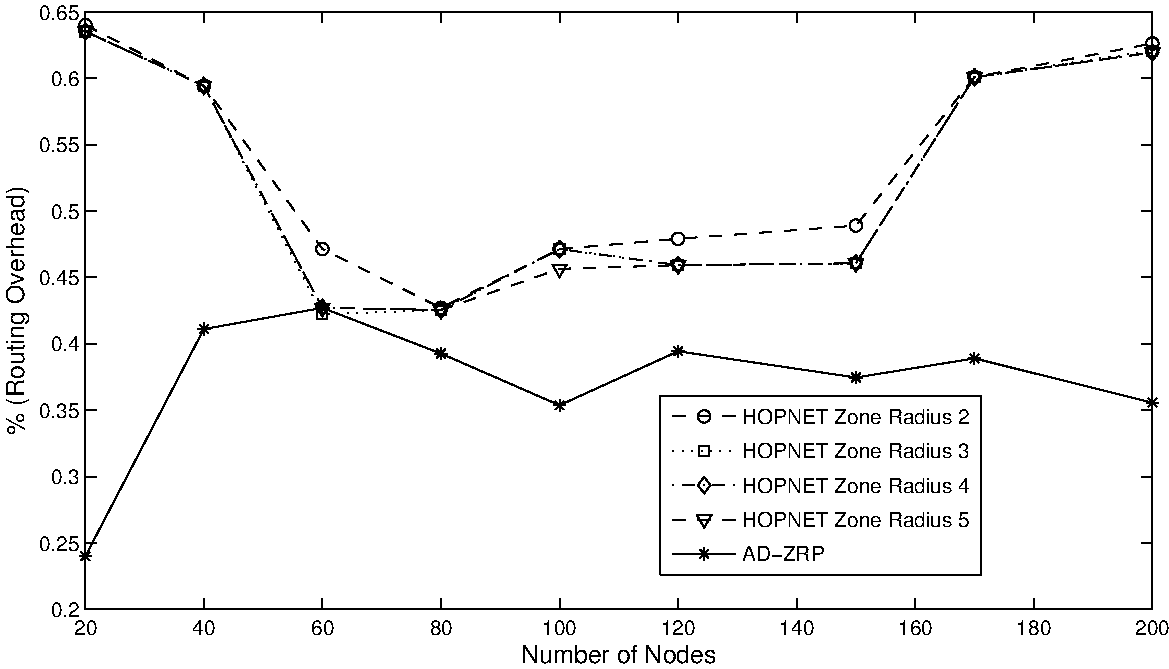
\includegraphics[width=245pt]{fig/routing_overhead.pdf}
\end{tabular}
\caption{Routing Overhead}
\label{routing_overhead}
\end{figure}

\section{Conclusion}
\label{conclusion}

In this paper, we have presented AD-ZRP, a routing algorithm based on the HOPNET algorithm.
As a routing algorithm inspired by ACO, AD-ZRP uses pheromone as a metric to make routing decisions, and uses heuristic information for pheromone deposit ratio.
We have evaluated and compared our algorithm to the original HOPNET and obtained better results in terms of data delivery ratio, routing overhead, and congestion avoidance for environments of dynamic topology.
Our proposal focuses primarily on routing overhead to reduce the amount of control packets from the network to require less effort in communication.
In fact, AD-ZRP achieves these results through the routing method based on \emph{dynamic zones} which tends to keep the best routes in terms of connectivity without significant losses in the data delivery ratio.
These \emph{dynamic zones} allow us to improve the routing and to avoid the necessity of complex structures and procedures thus increasing the efficiency and reducing the routing complexity for WSNs.

In future work, we are planning to extend the analysis of our algorithm in a real WSN environment to improve the experimental scenarios of dynamic topologies.
We also wish to focus on the heuristics information such as latency, location, coverage, and energy consumption.

\bibliographystyle{IEEEtran}
\bibliography{paper}

\end{document}

